\subsection{Task 2: Harnessing imperfect data and configuration to improve robustness.}

Regarding the identified robustness issues found in \textbf{Task 1}, we plan to improve the robustness of the trained model $\mathcal{M}$ on the top-$Q$ perturbation strategies via contrastive robust learning (CRL). In this project, CRL aims to learn the robust representation by contrasting similar (positive) and dissimilar (negative) objects instead of learning to recognize them individually. We intend to extend the contrastive learning paradigm into three imperfect DNN scenarios: perturbed inputs, perturbed outputs, and configuration variance. 

Regarding the scenarios with different perturbation strategies, the given target data are applied to its fitted contrastive loss: 
(1) Adversarial loss is addressed in the perturbed inputs scenario that the contrastive pair is the target inputs and their following perturbed inputs which can be viewed as positive pairs; 
(2) Label-flipping loss is computed on the variations of the noisy labels to reduce the effects of imprecise labels, by which the ground-truth labels and noisy labels can be viewed as negative pairs; 
(3) Configuration loss is utilized to update our target model to be trained dissimilar to the perturbed model which is proven to be less robust.
Furthermore, we propose a $mixture-loss$ for CRL, which is a concise loss function to enhance the robustness of the model in addressing the three scenarios together.

\begin{figure}[!h]
    \centering
    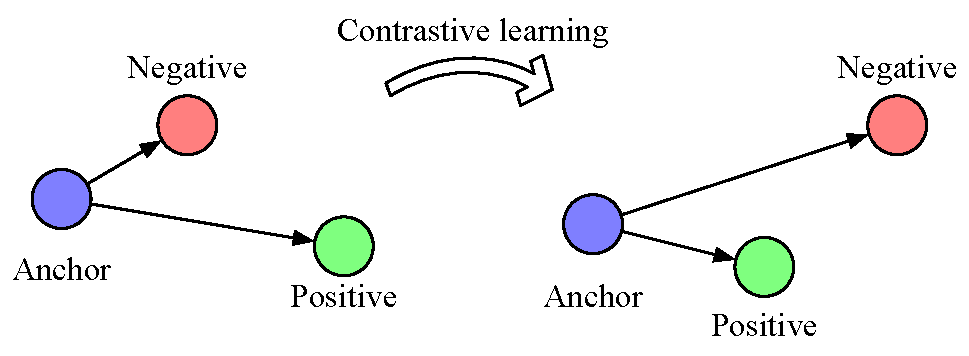
\includegraphics[width=9cm]{fig/contra.pdf}
    \caption{Contrastive learning}
    \label{fig:goal2}
\end{figure}

\textbf{Contrastive loss} Following the above definition of the model $f_{\Theta}: \mathbb{X} \rightarrow \mathbb{Y}$, the loss function quantifies the differences between the expected outcome and the model produced one. Contrastive loss obtains the outputs of the network for the positive (similar) examples of the same class, which is expected to be minimized, and contrasts that with the distance to negative (dissimilar) examples, which is expected to be maximized. Formally, the contrastive loss is present for the similar and dissimilar cases in Equation~\eqref{eq:contra}:
\begin{equation}\label{eq:contra}
    \mathcal{L}_{ct}(x_i,x_j) = \left\{\begin{matrix}
                          \|f_{\theta}(x_i)-f_{\theta}(x_j)\|_{\mathtt{p}} + \gamma,    & ct=+ \\
                          - \|f_{\theta}(x_i)-f_{\theta}(x_j)\|_{\mathtt{p}} + \gamma,  & ct=-
    \end{matrix}\right.
\end{equation}
where $\gamma$ is a hyper-parameter that is configured for the offset to the distances of a positive ($ct=+$) or negative ($ct=-$) pair, and the $x_j$ and $x_i$ are sampled from or generated by the strategies in $\mathbb{X}$ or $\hat{\mathbb{X}}$. 

\textbf{Adversarial loss} Given one target training input (anchor input) $x\in\mathbb{X}$, we can generate the corresponding perturbed input $\hat{x} \in \hat{\mathbb{X}}$ via the perturbation strategy $\omega$. 
Following the Equation~\eqref{eq:contra}, in Equation~\eqref{eq:adv}, we set every original input and its perturbed one as a positive pair ($x_i,\hat{x_i}$); we set original data from dissimilar classes ($x_i,x_j$), the original data from perturbed dissimilar classes ($x_i,\hat{x_j}$) and two perturbed dissimilar data ($\hat{x_i},\hat{x_j}$) as negative pairs. And we aim to find the model configuration ($\Theta$) for achieving the guaranteed robustness to the perturbed inputs.

\begin{equation}\label{eq:adv}
    \mathcal{L}_{adv} = \mathcal{L}_{+}(x_i,\hat{x_i}) + \mathcal{L}_{-}(x_i,x_j) + \mathcal{L}_{-}(x_i,\hat{x_j})  + \mathcal{L}_{-}(\hat{x_i},\hat{x_j}) 
    % \sum_{(x,y) \in (\mathbb{X},\mathbb{Y})}\max (0, \mathcal{L}(f_{\Theta}(x),y)-\mathcal{L}(f_{\Theta}(\hat{x}),y))
\end{equation}

\textbf{Label-flipping loss} Given one target training output (anchor output) $y\in\mathbb{Y}$, we can generate the corresponding perturbed output $\hat{y} \in \hat{\mathbb{Y}}$ via the perturbation strategy $\omega$. In practice, it is difficult to distinguish all noisy labels in a large dataset. $\mathcal{L}_{flip}$ is trying to reduce the contribution of noisy label ($\hat{y}$) to the model. The term in Equation~\eqref{eq:flip} is a negative pair, where $\lambda$ provides benefits for training with a noisy label that makes it hard to map with the noisy pattern. 
\begin{equation}\label{eq:flip}
    \mathcal{L}_{flip} = \sum_{(x,y) \in (\mathbb{X},\mathbb{Y})} \max (0, \mathcal{L}(f_{\theta}(x),y)-\mathcal{L}(f_{\theta}(x),\hat{y}))\\ 
\end{equation}

\textbf{Configuration loss} Given the less robust model ($\hat{\mathcal{M}}$) studied and generated from \textbf{Task 1}, intuitively, we cannot linearly calculate which configuration setting is degrading the robustness of the model. $\mathcal{L}_{conf}$ denotes the configuration loss, which contrasts the mapping context, to find the model configuration ($\Theta$) farther apart from the less robust and perturbed model $\hat{\mathcal{M}}$.
\begin{equation}
    \mathcal{L}_{conf} = \sum_{(x,y) \in (\mathbb{X},\mathbb{Y})} \max (0, \mathcal{L}(f_{\theta}(x),y)-\mathcal{L}(f_{\hat{\theta}}(x),y))
\end{equation}

\begin{equation}
    % \mathcal{L}_{mix} = \sum_{(x,y) \in (\mathbb{X},\mathbb{Y})} \max (0, \mathcal{L}(f_{\Theta}(x),y)-\mathcal{L}(f_{\hat{\Theta}}(\hat{x}),\hat{y}))
    \mathcal{L}_{mix} = \mathcal{L}_{adv} - \mathcal{L}^{flip}-\mathcal{L}^{conf}
\end{equation}





% In Figure~\ref{fig:goal2}, contrastive pertaining, which extends from SimCLR, for unsupervised learning 
% We aim to learn the robust feature representation from the data, in which the resulting training mini-batch $\{(x_i,y_i)\}_{i=1}^N$ of the pairs $x_i$ to its label $y_i$ contains $N$ pairs. Each pair of the data is mapped in the latent space as a low-dimensional representation ($z_i$) by learning an encoder ($EC$) and a target model ($\mathcal{M}$), where 
% SSL has been recently studied from multiple domains~\cite{chen2020big} and explored in various strategies (e.g., generative models~\cite{odena2016semi,shu2022reducing}, pseudo-labelling~\cite{arazo2020pseudo}), which benefits both from transductive (i.e., label the unlabelled data to learn) and inductive (i.e., guide the inputs to the outputs as a mapping function with high generality).



% CAP retrieves and discriminates the features from the labelled ($\mathcal{D}^l$) and unlabelled ($\mathcal{D}^u$) data for semi-supervised labelling, which significantly decreases the manually labelling workload and discloses imperceptible patterns by humans. 
% The active sampling is conducted $k$-th iteration with the selected data on top of contrastive un-supervised clustering, which introduces the human intellectual concept to secure the self-supervised contrastive learning model to be more reliable when countering the ambiguous data (i.e., a small amount of the weakly labelled data are assumed to be located on the boundary between two different clusters).
% First, we train the learning model using the existing labelled samples ($\mathcal{D}^l_0$), and for the ($i+1$)-th iteration of data selection, a portion of unlabelled data ($\mathcal{D}^l_{i+1} \subseteq \mathcal{D}^u_{i+1}$), are selected to be automatically labelled by the model that trained at the $i$-th iteration, where $\mathcal{D}^u_{i+1} = \mathcal{D}^u_i \backslash \mathcal{D}^l_i$. The labelled samples during each iteration are incrementally added to the training set (i.e., $\bigcup^i_{j=0}\mathcal{D}^l_j\subseteq \mathcal{D}^l$) to retain the model and continuously improve its performance. 

% Regarding the data issues from Equation~\eqref{eq1} and Equation~\eqref{eq3}, CAP countermeasures are corresponding to \textcolor{red}{(To be extended by equation 1 and 2)}: 
% \begin{itemize}
%     \item Perturbed inputs: Considering benign samples are commonly perturbed as adversarial samples and lucked in the training set, we aim to distinguish the benign samples and adversarial ones through contrastive active learning.
%     \item Noisy labels: we use contrastive active learning to automatically fix the wrong labels. 
% \end{itemize}

